\section{Related Works}
\label{sec:related_works}
\subsection{Safe Reinforcement Learning}
Safe RL is commonly formulated as a Constrained Markov Decision Process (CMDP)\cite{CMDP}, which seeks to optimize agent rewards while adhering to safety constraints. Solutions to CMDPs cam be categorized into two primary approaches: Primal-Dual Optimization (PDO)\cite{Primal_Dual_Optimization} and Constrained Policy Optimization (CPO). PDO predominantly relies on Lagrangian relaxation, a technique that iteratively updates primal and dual variables to manage constraints. Within this category, the Lagrangian method\cite{lagrangian} is a useful technique that transforms constrained optimization problems into their unconstrained counterparts. It offers straightforward implementation and avoids the computational burden of complex Hessian matrix computations. In contrast, Achiam \textit{et al.} introduced the Constrained Policy Optimization (CPO) algorithm\cite{CPO}, which employs quadratic constraint optimization to handle constraints within RL. While CPO provides an approximation to constrained optimization, it generally entails higher computational costs compared to Lagrangian-based methods. Moreover, the performance of CPO can be affected by approximation errors and sampling inaccuracies.

However, traditional Lagrangian methods are susceptible to oscillations, particularly when operating near constraint boundaries\cite{stooke2020responsive}. Furthermore, these methods are sensitive to the initial setting of the Lagrange multiplier $\lambda$. Our method addresses these limitations by directly learning risk and entropy weights at each step, thereby dynamically balancing exploration and risk aversion in response to varying traffic scenarios.


\begin{figure*}[htbp]
    \centering
    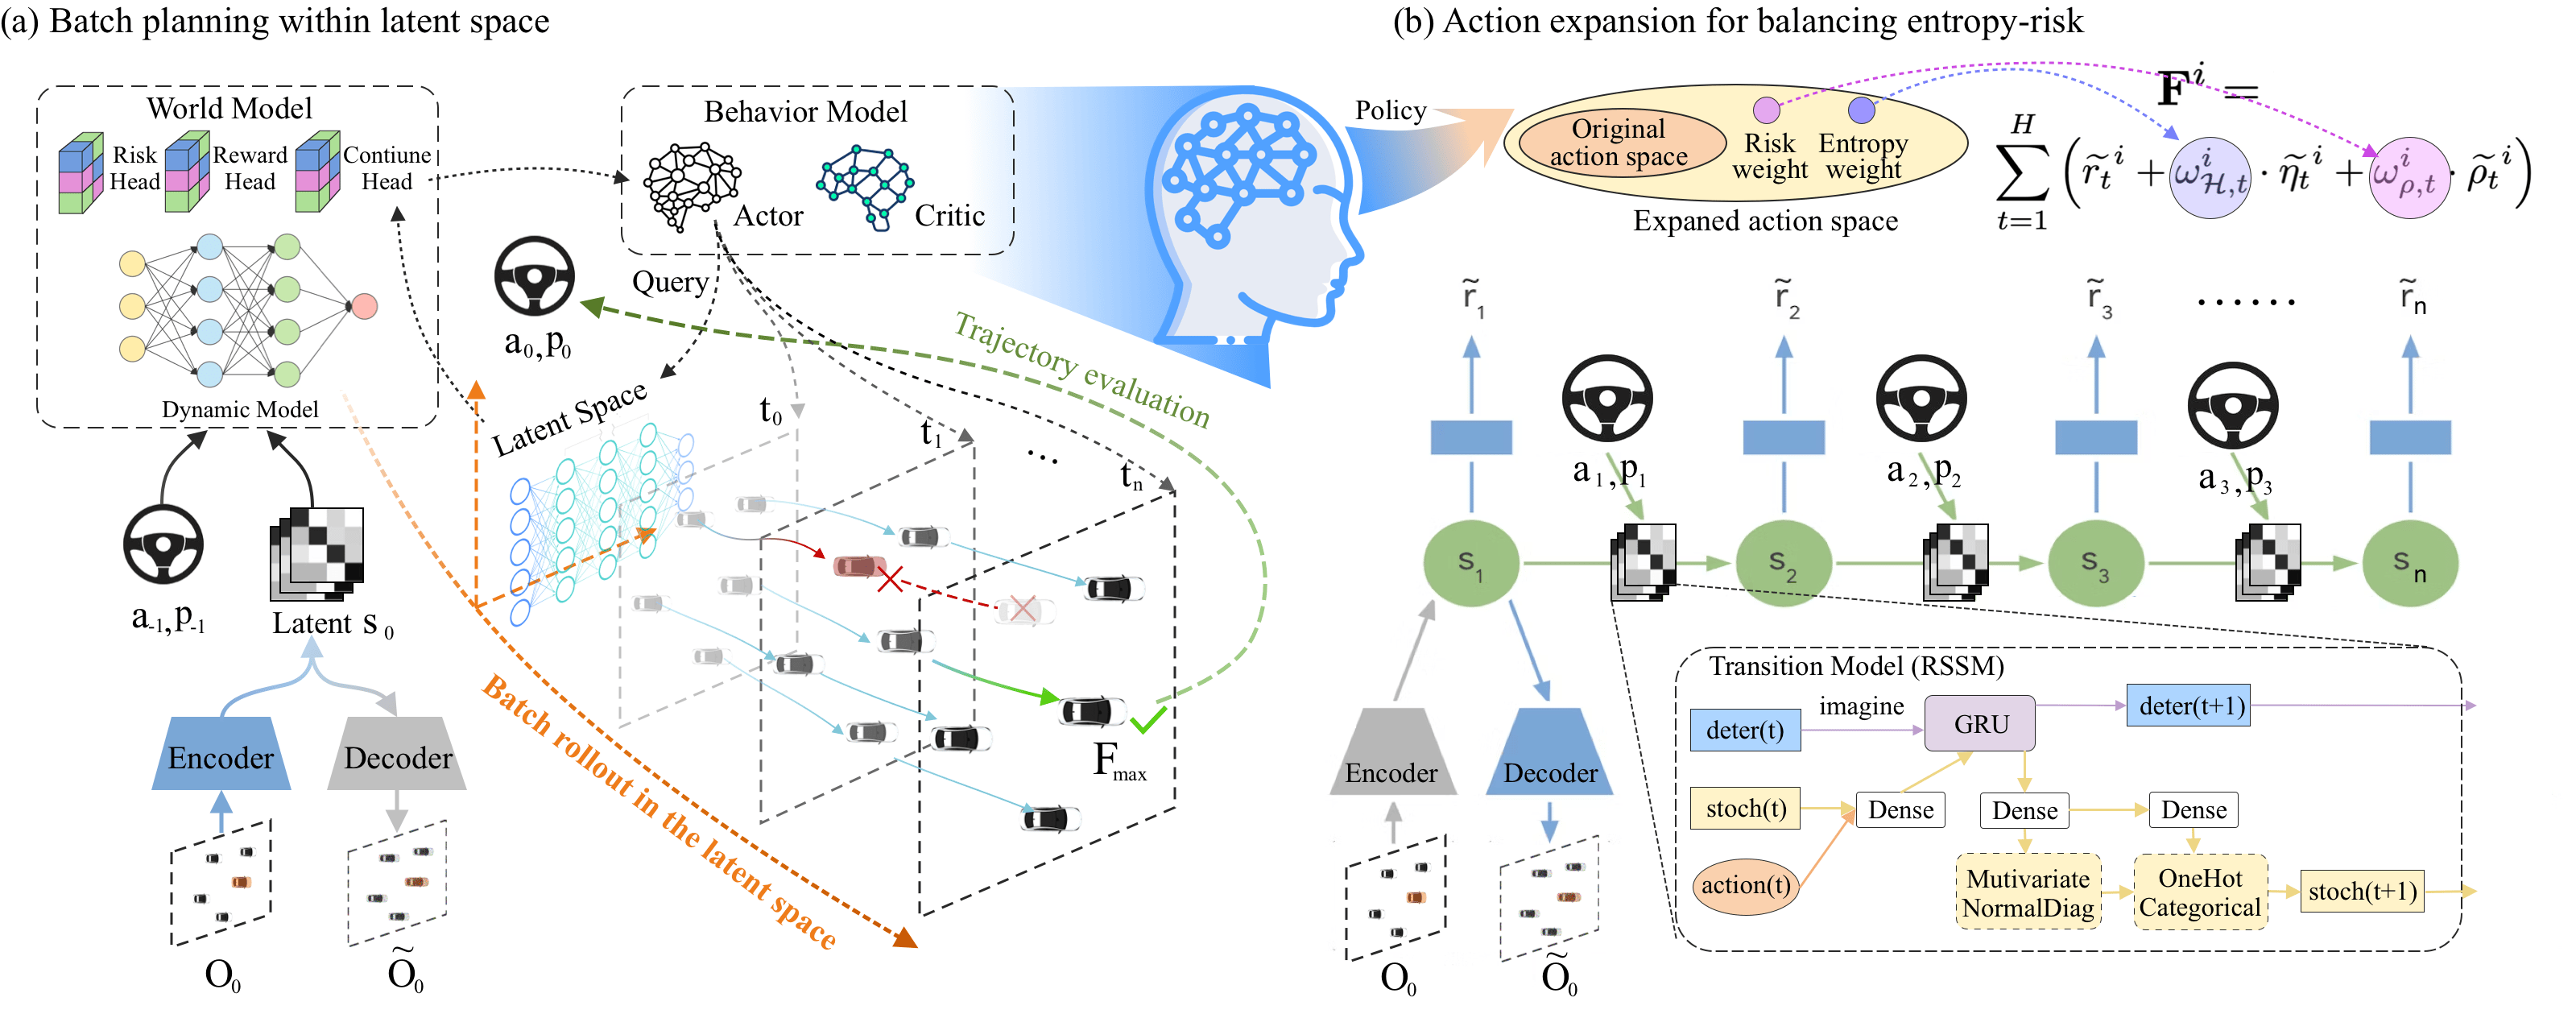
\includegraphics[width=\textwidth]{fig/Algo.png}
    \caption{Framework of the RiskDreamer algorithm. (a) Batch planning within latent space. (b) Action expansion for balancing entropy-risk. }
    \label{fig:algo}
\end{figure*}


\subsection{Planning in Latent Space}
World model\cite{ha2018world} has succeed in learning potential dynamic models capable of inferring future latent representations of the environment. The Dreamer algorithm series\cite{dreamer},\cite{dreamerv2},\cite{dreamerv3}, utilized model-based reinforcement learning through its recurrent state-space model (RSSM)\cite{RSSM}. By constructing internal world models, the algorithm enables agents to learn in virtual environments, reducing required physical interactions and enhancing both efficiency and safety in real-world applications. However, the greedy MDP behavior model in DreamerV3 struggles with long sequence decision-making, leading to suboptimal performance in continuous action sequence tasks.
Huang \textit{et al.} extended DreamerV3\cite{dreamerv3} by incorporating the Lagrangian method and Curiosity Cross-Entropy Method\cite{CCEM} to develop SafeDreamer\cite{safedreamer}. However, similar to most Lagrangian-based approaches, its performance is highly sensitive to the cost threshold \cite{gao2024enhance}. Wen \textit{et al.} \cite{CCEPETS} proposed an algorithm based on the constrained cross-entropy method, which optimizes constraints through iterative updates of elite samples. Despite its effectiveness, this approach incurs high computational costs. In contrast, our method improves planning efficiency by concurrently generating multiple imagined trajectories in latent space.
\subsection{Naturalistic Driving Simulation}
The training environment is crucial for reinforcement learning, especially in the context of autonomous driving. Current traffic simulations typically rely on either replayed data or homogenous heuristic models to emulate background traffic agents.
In a review of RL literature for autonomous vehicles, Noaeen \textit{et al.}\cite{noaeen2022reinforcement} identified that few papers incorporated simulations with diverse vehicle types. Additionally, They also noted the absence of explicit discussions about car-following parameters in autonomous vehicles RL research. Schrader \textit{et al.}\cite{sumoclibration} calibrates the parameters for each pair of car-following vehicles. However, this calibration is based on pairs of following vehicles, lacking calibration for multi-vehicle interactive movements. Yan \textit{et al.}\cite{NDE} employed neural networks to simulate the behavior of traffic agents, thereby achieving macro-level statistical realism. However, the safety mapping network mechanism they utilized does not guarantee the plausibility of microscopic traffic trajectories. 
By contrast, our method generates heterogeneous traffic agents with realistic behavior and statistics, enhancing the realism and challenge of the training environment. 